% ======================================================================
% article.tex — master document for the "Reusable by Construction" article
% Build:  make            (or latexmk -pdf article.tex)
% Sources: see SOURCE_MAP.md; evidence: see EVIDENCE.md
% ======================================================================
\documentclass[11pt]{article}

\usepackage[margin=1in]{geometry}
\usepackage{amsmath,amssymb,amsthm}
\usepackage{bm}
\usepackage{booktabs}
\usepackage{tabularx}
\usepackage{array}
\usepackage{graphicx}
\usepackage{xcolor}
\usepackage{siunitx}
\usepackage{listings}
\usepackage[font=small,labelfont=bf]{caption}
\usepackage[round,numbers]{natbib}
\usepackage[colorlinks=true,linkcolor=blue,citecolor=blue,urlcolor=blue]{hyperref}
\usepackage{microtype}
\usepackage{tikz}
\usetikzlibrary{arrows.meta,positioning,fit,backgrounds,calc,shapes.geometric}

% ---------------------------------------------------------------- shortcuts
\newcommand{\R}{\mathbb{R}}
\newcommand{\E}{\mathbb{E}}
\newcommand{\Prob}{\mathbb{P}}
\newcommand{\Cvar}{\mathrm{CVaR}}
\newcommand{\ind}{\mathbb{I}}
\newcommand{\xx}{\mathbf{x}}
\newcommand{\dd}{\,\mathrm{d}}
\newcommand{\pdd}[2]{\frac{\partial #1}{\partial #2}}
\newcommand{\pddt}[2]{\frac{\partial^{2} #1}{\partial #2^{2}}}
\newcommand{\erfc}{\operatorname{erfc}}
\newcommand{\norm}[1]{\left\lVert #1 \right\rVert}
\newcommand{\Lpde}{\mathcal{L}_{\mathrm{PDE}}}
\newcommand{\Lic}{\mathcal{L}_{\mathrm{IC}}}
\newcommand{\Lbc}{\mathcal{L}_{\mathrm{BC}}}
\newcommand{\Ldata}{\mathcal{L}_{\mathrm{data}}}
\newcommand{\code}[1]{\texttt{#1}}

\lstset{
  basicstyle=\ttfamily\small,
  breaklines=true,
  columns=fullflexible,
  keepspaces=true,
  frame=single,
  framerule=0.3pt,
  rulecolor=\color{gray!50},
  backgroundcolor=\color{gray!5},
  aboveskip=0.6em,
  belowskip=0.6em
}

\title{\bfseries Reusable by Construction:\\[2pt]
\large An AI-Assisted Path from Research Scripts to a Verified\\
Groundwater Remediation Stack}
\author{S. Lucero\\[2pt]
\small with the Pi coding agent (DeepSeek models)}
\date{\today}

\begin{document}
\maketitle

% ======================================================================
% 00-abstract.tex
% ======================================================================
\begin{abstract}
\noindent
Research code usually becomes reusable by accident, if at all. We report a
different path: a groundwater-remediation project in which the code was made
reusable \emph{by construction}, one failure at a time, with an AI coding agent
(the Pi harness running DeepSeek models) doing most of the implementation,
testing and record-keeping. The scientific stack is a verified
advection--dispersion sandbox, a batched finite-volume Darcy/transport solver, a
chance-constrained pump-and-treat optimizer, and 1D/2D/3D experiments.
The reusable artifacts are less glamorous: one NumPy reference implementation
with a parity-tested torch backend, configuration manifests that record seed,
device, dtype and git revision, gate suites that turn physical assumptions into
go/no-go conditions, a seed-sweep harness that reports medians with their spread,
and an artifact-first remote runner that keeps the results of a run that dies.
We show that these mechanisms changed conclusions, not just style: a
single-seed ``32\% improvement'' became a negative result, an FNO that scored
worse than predicting zeros became a 1.5\% operator on one seed (3\% median), a policy that passed its
own reliability gate failed on the independent NumPy reference, and a 3D paper
preset reproduced on a third machine with a different BLAS. We also report where
the agent was confidently wrong, and argue that the useful division of labour is
not ``human writes, AI types'' but \emph{human owns the gates, agent owns the
iteration count, and the repository owns the memory}.
\end{abstract}

\vspace{0.5em}
\noindent\textbf{Keywords:} research software; reproducibility; physics-informed
neural networks; Fourier neural operators; stochastic optimization;
AI-assisted development.

% ======================================================================
% 01-intro.tex
% ======================================================================
\section{Introduction}
\label{sec:intro}

Three numbers illustrate why this article is about software rather than
physics.

The first is a Fourier neural operator (FNO) with relative $L^2$ error
$0.973$. It had been recorded as a weak result. It was not weak: because the
metric is normalized by the target norm, a predictor of all zeros scores exactly
$1.0$, so the operator was \emph{worse than predicting nothing}. The input was
two spatially constant parameter channels; a pointwise lift followed by spectral
layers that multiply Fourier coefficients can only produce a constant output.
The architecture was structurally incapable of representing a front, and no
amount of training could fix it.

The second is a physics-informed neural network (PINN) reported at
$1.35\times10^{-2}$ full-grid error and $8.0\times10^{-3}$ in the interior. It
was the best of five seeds. At fixed hyperparameters the same configuration
spans $1.17\times10^{-2}$ to $8.14\times10^{-2}$---a factor of seven---and the
median interior error is $1.42\times10^{-2}$, not below the $10^{-2}$ target the
result was said to meet.

The third is a claimed $5\times$ GPU speedup that had never been measured. When
the launch count was finally instrumented, one evaluation issued $4{,}022$
batched matrix--vector products, $1.7\times$ the number the optimization plan
had assumed. The speedup may still be real; the point is that it was being
\emph{planned} as if it were a result.

None of these is a modelling failure. Each is a failure of the process that
decides what counts as evidence: a metric without a baseline, a run without
repetition, a claim without an instrument. The response could have been a
refactor. Instead, this project accumulated \emph{gates}: a trivial-predictor
guard that makes an FNO worse than zeros fail fast; a seed-sweep harness that
refuses to compare unpaired runs; a backend-parity suite that treats a numerical
disagreement as a bug; an artifact-first remote runner that keeps the results of
a run that dies. The gates are the reusable code.

\paragraph{Why AI matters here.}
Writing research software is usually a choice between doing the experiment and
doing the software hygiene, and the experiment wins. The standard remedies---
version control, tests, continuous integration, documented environments---are
well known \citep{wilson2014best,sandve2013ten}, but they are labour, and the
labour is repetitive rather than creative. An agent that can read the repository,
run the test, read the failure, edit the file, rerun, and write down what
happened changes the marginal cost of that labour. Recent work on agents that
act through tools and on benchmarks built from real repository issues makes the
same point from the other direction: the hard part is not generating a patch,
it is closing the loop against an executable check
\citep{yao2023react,jimenez2024swebench}.

This article is an experience report from one project in which that loop was
closed with the Pi coding agent\footnote{\url{https://pi.dev/}} running DeepSeek
models.\footnote{\url{https://www.deepseek.com/}} The agent performed most of
the edits, test runs, benchmark harnesses and documentation updates. The human
chose the gates, rejected the tempting numbers, and wrote the final judgements.
We are explicit about this division because it is the article's main claim.

\paragraph{Thesis.}
Reusability is not a property of a directory layout or a test count. It is the
accumulation of falsifiable gates, written memory, and one reference
implementation---and an AI agent made that accumulation cheap enough to do on
every failure instead of once at the end.

\paragraph{Claims.}
The article argues three claims, each with evidence from the repository:
\begin{enumerate}
  \item \textbf{Reusability is measurable.} The same policy reproduces on a
        third machine, the NumPy and torch backends agree to $10^{-10}$ and
        select the same policy, and a certificate on 400 unseen scenarios
        survives a redraw.
  \item \textbf{The reusable artifacts came from a repeatable loop.} Every
        mechanism in \S\ref{sec:mechanisms} and every guard in
        \S\ref{sec:failures} is traced to a specific defect and a commit; none
        arrived from a big-bang rewrite.
  \item \textbf{AI's contribution was verification throughput and memory, not
        code volume.} The failure catalogue includes cases where the agent was
        confidently wrong, and the human protocol that caught them is part of
        the method.
\end{enumerate}

\paragraph{Contributions.}
(i) A concrete account of five reusability mechanisms in a computational
hydrology stack: reference/batched parity, configuration manifests, gates,
statistical harnesses, and artifact-first remote execution. (ii) A failure
catalogue in which each defect became a permanent guard, with the commit and
the test that pins it. (iii) A set of results that survive independent
re-derivation, including one that fails its own in-run certificate. (iv) A
practical account of what an AI agent did well and where it failed.

\paragraph{Roadmap.}
\S\ref{sec:case} fixes the scientific setting. \S\ref{sec:method} describes the
AI-assisted loop and the artifacts that serve as memory. \S\ref{sec:mechanisms}
presents the five mechanisms. \S\ref{sec:failures} is the failure catalogue.
\S\ref{sec:results} reports the results that survived, with their caveats.
\S\ref{sec:discussion} discusses the collaboration and its threats to validity,
and \S\ref{sec:conclusion} concludes. Appendices collect gate definitions,
repository layout and full tables.

% ======================================================================
% 02-case.tex — the scientific setting, condensed from TEX/formulation.tex
% and TEX/optimization.tex. Full derivations: see those files and Appendix A.
% ======================================================================
\section{The scientific setting}
\label{sec:case}

The project has two halves: neural surrogates for a contaminant-transport
equation, and a stochastic optimization layer that decides pumping rates under
geological uncertainty. Both are standard; we summarize only what the gates
need.

\subsection{One-dimensional sandbox and neural surrogates}
\label{sec:case-1d}

The verification problem is the dimensionless advection--dispersion equation
(ADE) for a conservative solute in a homogeneous, isotropic aquifer,
\begin{equation}
\pdd{u}{\tau}+\pdd{u}{\xi}
=\frac{1}{\mathrm{Pe}}\,\pddt{u}{\xi},
\qquad (\xi,\tau)\in(0,1)\times(0,\tau_{\max}],
\label{eq:ade}
\end{equation}
with step inlet and clean initial state,
\begin{equation}
u(\xi,0)=0,\qquad u(0,\tau)=1,\qquad u(1,\tau)=0,
\label{eq:bc}
\end{equation}
where $\xi=x/L$, $\tau=tv/L$ is measured in pore volumes, $u=C/C_0$, and
$\mathrm{Pe}=vL/D$. The closed-form Ogata--Banks solution
\citep{ogata1961solution}
\begin{equation}
u_{\mathrm{ref}}(\xi,\tau)=\frac12\left[
\erfc\!\left(\frac{(\xi-\tau)\sqrt{\mathrm{Pe}}}{2\sqrt{\tau}}\right)
+e^{\mathrm{Pe}\,\xi}\,
\erfc\!\left(\frac{(\xi+\tau)\sqrt{\mathrm{Pe}}}{2\sqrt{\tau}}\right)
\right]
\label{eq:ogata}
\end{equation}
is the ground truth. The shipped configuration uses $\mathrm{Pe}=20$,
$\tau_{\max}=0.5$ and a $256\times256$ test grid.

\paragraph{PINN.} A multilayer perceptron $u_\theta(\xi,\tau)$ ($\tanh$ hidden,
sigmoid output) minimizes
\begin{equation}
\mathcal{L}(\theta)=\lambda_{\mathrm{PDE}}\Lpde
+\lambda_{\mathrm{IC}}\Lic+\lambda_{\mathrm{BC}}\Lbc,
\label{eq:loss}
\end{equation}
with the PDE residual
$\mathcal{R}_\theta=\pdd{u_\theta}{\tau}+\pdd{u_\theta}{\xi}
-\mathrm{Pe}^{-1}\pddt{u_\theta}{\xi}$
formed by automatic differentiation and each term a mean square over resampled
collocation points. The best configuration uses a \emph{hard} ansatz that
satisfies the initial and outlet conditions identically and the inlet up to a
short ramp,
\begin{equation}
u_\theta(\xi,\tau)=(1-\xi)\,s(\tau)
+\xi(1-\xi)\,s(\tau)\,\mathrm{NN}_\theta(\xi,\tau),
\qquad s(\tau)=1-e^{-\tau/\varepsilon},
\label{eq:hardbc}
\end{equation}
with $\varepsilon=10^{-3}$. Both terms carry $s(\tau)$, so $u_\theta(\xi,0)=0$;
both carry $(1-\xi)$ or $\xi(1-\xi)$, so $u_\theta(1,\tau)=0$. Only the inlet is
approximate: $u_\theta(0,\tau)=s(\tau)\to1$ for $\tau\gg\varepsilon$.

\paragraph{Two artefacts worth knowing.} First, the step-inlet problem is
discontinuous at the corner $(\xi,\tau)=(0,0)$: the initial condition says
$u=0$, the inlet says $u=1$, and the reference returns $1$. Every continuous
ansatz that honors the initial condition returns $0$, so the pointwise error at
the corner is exactly one and a thin band around it is contaminated. This is a
metric artefact, not a network bug, and it is why two metrics are always
reported: the full-grid relative $L^2$ error and a corner-excluded interior
error over $\{\xi>0.05,\ \tau>0.05\}$. Second, the ramp contributes
$s'(0)=1/\varepsilon$, so
\begin{equation}
\max_{\xi,\tau}|\mathcal{R}_\theta|\gtrsim 1/\varepsilon
\label{eq:resfloor}
\end{equation}
\emph{independently of the weights}. At $\varepsilon=10^{-3}$ the corner
residual is $1.0\times10^{3}$ at initialization and after training, and on every
seed. A global residual maximum is therefore a useless diagnostic here; only
band means are meaningful.

\paragraph{FNO.} The Fourier neural operator \citep{li2020fourier} learns the
solution operator from parameters to the concentration field: a lifting MLP,
spectral convolution layers with $k_{\max}$ retained modes, and a projection
MLP. The 1D campaign uses a family of $(v,D)$ scenarios and evaluates against
\eqref{eq:ogata}. The architecture's input representation turns out to be the
whole story (\S\ref{sec:failures}).

\subsection{Two- and three-dimensional pump-and-treat}
\label{sec:case-opt}

The remediation problem couples steady Darcy flow to advective--dispersive
transport. With transmissivity $T=Kb$, head $h$, recharge $W$ and extraction
rates $q_i$ at wells $\xx_i$,
\begin{equation}
-\nabla\cdot\bigl(T(\xx)\nabla h\bigr)
=b\,W(\xx)-\sum_{i=1}^{n_w}q_i\,\delta_\varepsilon(\xx-\xx_i),
\label{eq:darcy}
\end{equation}
where $\delta_\varepsilon$ is a normalized Gaussian well kernel. Transport is
\begin{equation}
\phi R\,\pdd{C}{t}
=\nabla\cdot(\phi\mathbf{D}\nabla C)
-\nabla\cdot(\phi\mathbf{v}C)
-\sum_i q_i C(\xx_i)\delta_\varepsilon(\xx-\xx_i)+s(\xx,t),
\label{eq:transport}
\end{equation}
with velocity $\mathbf{v}=-K\nabla h/\phi$, dispersion tensor $\mathbf{D}$,
retardation $R$ and source $s$. Implicit Euler with first-order upwinding makes
the transport operator linear in $q$ and admits an exact discrete adjoint.

\paragraph{Random conductivity.} The primary random input is a log-normal field
\begin{equation}
K(\xx,\omega)=K_0\exp\!\bigl(G(\xx,\omega)\bigr),
\qquad
G=m_G+\sum_{n=1}^{N_{KL}}\sqrt{\lambda_n}\,\varphi_n(\xx)\,\xi_n(\omega),
\label{eq:kl}
\end{equation}
with $\xi_n\sim\mathcal{N}(0,1)$ and $(\lambda_n,\varphi_n)$ the eigenpairs of
an exponential covariance with variance $\sigma_G^2$ and correlation length
$\ell$ \citep{ghanem1991stochastic}. The benchmark uses
$\sigma_G=0.65$, $\ell=15$\,m, a 95\% variance truncation
($n_{KL}=1529$ at $160\times96$), nine candidate wells on a hexagonal lattice,
and a $10\ \mathrm{m^3/d}$ source at $100\ \mathrm{mg/L}$ for 3650 days.

\paragraph{The stochastic program.} The decision is a vector of nonnegative
pumping rates $\mathbf{q}$ in a convex admissible set $\mathcal{Q}$ (per-well
capacity, total budget, drawdown). The cost $J(\mathbf{q},\omega)$ combines
pumping energy, treatment, residual contamination and cleanup time. Compliance
is a random constraint $G(\mathbf{q},\omega)\le0$ at a monitoring line over the
final 20\% of the horizon, and the problem is
\begin{equation}
\min_{\mathbf{q}\in\mathcal{Q}}\ \E\bigl[J(\mathbf{q},\omega)\bigr]
\quad\text{s.t.}\quad
\Prob\bigl(G(\mathbf{q},\omega)\le0\bigr)\ge1-\alpha,
\label{eq:chance}
\end{equation}
with $\alpha=0.05$ and a head constraint handled analogously. The expectation
is approximated by sample-average approximation (SAA) over $M_{\text{train}}$
scenarios, and the chance constraint by a Rockafellar--Uryasev CVaR penalty
\citep{rockafellar2000optimization,shapiro2009lectures}. The search is a pattern
search with capacity projection and a batched compass sweep
\citep{audet2006mesh}. The full program, variants and algorithm discussion are
in \texttt{TEX/optimization.tex} and \texttt{TEX/SolvingAlgorithms.tex}.

\subsection{What counts as a result}
\label{sec:case-result}

The project uses four evidence classes, and every quantitative statement in
this article is labelled with one:
\begin{enumerate}
  \item \textbf{Derived}: true by construction (e.g.\ the $1/\varepsilon$
        residual floor), so seed-independent.
  \item \textbf{Multi-seed}: a median over $N\ge5$ seeds with its interquartile
        range, and a paired comparison for any variant.
  \item \textbf{Gated}: a run that clears a named threshold on a named artifact
        (mass balance, retained variance, backend parity, reliability).
  \item \textbf{Certified}: a policy re-evaluated out of sample, with a Wilson
        interval \citep{wilson1927probable}, not a bare fraction.
\end{enumerate}
The rest is \emph{preliminary} and is labelled as such. This taxonomy is the
article's unit of analysis: the mechanisms in \S\ref{sec:mechanisms} exist to
make each class cheap to produce, and the failures in \S\ref{sec:failures} are
cases where a weaker class was being reported as a stronger one.

% ======================================================================
% 03-method.tex — the AI-assisted reusability loop
% ======================================================================
\section{Method: the AI-assisted reusability loop}
\label{sec:method}

The project did not begin with a software-engineering plan. It began with a
research question and a set of runs whose results did not survive scrutiny. The
method emerged as a response to that: a six-step loop, executed by a human and
an agent, with the repository as the memory between turns.

\subsection{Roles}
\label{sec:roles}

\begin{table}[htbp]
\centering
\small
\begin{tabularx}{\textwidth}{@{}lX@{}}
\toprule
Actor & Responsibility in this project \\
\midrule
Human (PI/editor) &
Chooses the question and the acceptance threshold; decides which evidence
class a claim belongs to; rejects the best-seed number; writes and owns the
final prose; accepts or rejects a policy. \\
Pi (agent harness) &
Reads the repository; runs commands and tests; edits files; writes new tests,
harnesses and documentation; commits with the finding in the message; keeps the
memory files current. \\
DeepSeek (model) &
Proposes the diagnosis, the patch, the test and the summary that the harness
executes. Its output is a hypothesis until a gate passes. \\
Gemini (tertiary) &
Occasional research assistance and code review; not part of the loop. \\
\bottomrule
\end{tabularx}
\caption{Division of labour. The harness/model split matters: most of the
leverage came from the agent's ability to \emph{run} the check, not from a
single model completion.}
\label{tab:roles}
\end{table}

\subsection{The loop}
\label{sec:loop}

Each turn has six steps (Figure~\ref{fig:loop}):
\begin{enumerate}
  \item \textbf{Read the memory.} Before touching code, read \code{HUMAN.md},
        \code{Actions.md}, \code{Conclusions.md} and the relevant plan. This is
        the step that prevents re-learning an environment gotcha or
        re-litigating a closed question.
  \item \textbf{Reproduce the claim.} Run the command that produced the number,
        or the smallest version of it. A claim that cannot be reproduced is a
        bug report, not a baseline.
  \item \textbf{Change one thing.} The smallest reversible edit that could
        explain the failure---not a cleanup, not a refactor.
  \item \textbf{Run the gate.} A named threshold on a named artifact. If the
        gate does not exist yet, writing it is part of the change.
  \item \textbf{Record the finding.} Update the run log and the conclusions,
        including negative results. A finding that is not written where the next
        session will look did not happen.
  \item \textbf{Commit the finding.} The commit message states what was learned,
        not what files moved. This makes the history searchable by claim.
\end{enumerate}

\begin{figure}[htbp]
\centering
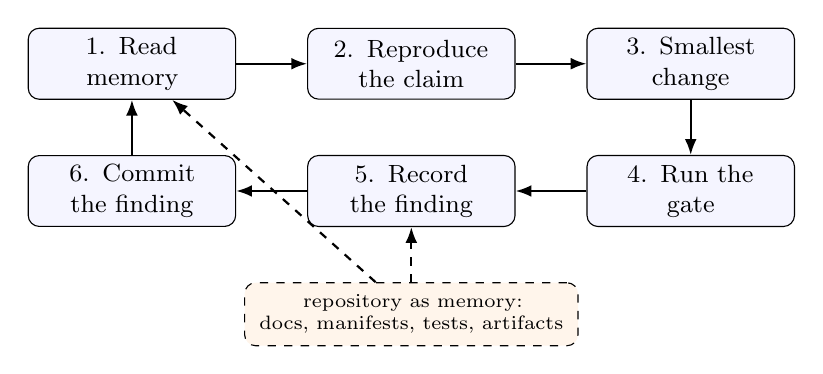
\begin{tikzpicture}[
  node distance=7mm and 9mm,
  box/.style={draw, rounded corners, align=center, font=\small,
              minimum height=9mm, text width=24mm, fill=blue!4},
  mem/.style={draw, dashed, rounded corners, align=center, font=\scriptsize,
              minimum height=8mm, text width=40mm, fill=orange!8},
  arrow/.style={-{Latex[length=2mm]}, thick}
]
\node[box] (read) {1. Read\\memory};
\node[box, right=of read] (repro) {2. Reproduce\\the claim};
\node[box, right=of repro] (change) {3. Smallest\\change};
\node[box, below=of change] (gate) {4. Run the\\gate};
\node[box, left=of gate] (record) {5. Record\\the finding};
\node[box, left=of record] (commit) {6. Commit\\the finding};
\node[mem, below=of record] (memory) {repository as memory:\\docs, manifests, tests, artifacts};
\draw[arrow] (read) -- (repro);
\draw[arrow] (repro) -- (change);
\draw[arrow] (change) -- (gate);
\draw[arrow] (gate) -- (record);
\draw[arrow] (record) -- (commit);
\draw[arrow] (commit.north) -- ++(0,4mm) -| (read.south);
\draw[arrow, dashed] (memory) -- (record);
\draw[arrow, dashed] (memory) -- (read);
\end{tikzpicture}
\caption{The loop. The dashed arrow is the property that makes it cumulative:
the repository, not the conversation, is the memory.}
\label{fig:loop}
\end{figure}

The loop is deliberately unoriginal; it is the scientific method with a commit
hook. What changed with AI is the \emph{cost per turn}. A human will run a
five-seed sweep once, at the end, when the paper is due. An agent will run it on
every candidate because the marginal cost of ``run the same command four more
times and tabulate the result'' is small. That is the entire mechanism behind
the negative result in \S\ref{sec:failures}: the $\tau$-ramp experiment was repeated
because repeating it was cheap, and the repetition destroyed the effect.

\subsection{Artifacts as memory}
\label{sec:memory}

Conversation context is volatile; a repository is not. The project therefore
keeps four kinds of memory, each written for a different reader.

\begin{table}[htbp]
\centering
\small
\begin{tabularx}{\textwidth}{@{}lX@{}}
\toprule
Artifact & Question it answers \\
\midrule
\code{HUMAN.md} & ``What will bite me when I come back?'' Environment gotchas,
wrong interpreter, out-of-memory, buffering, the corner artefact. Written for a
human under time pressure. \\
\code{Actions.md} & ``What was run, and what happened?'' A chronological run log
with numbers, artifact paths and negative results. \\
\code{Conclusions.md} & ``What is trustworthy, what is single-seed, what is
open?'' The evidence-class ledger for the whole project. \\
\code{USAGE.md} & ``How do I run this?'' Every entry point, its cost and its
outputs. \\
\code{runs/runtimes.jsonl} & ``What did it cost?'' One JSON record per run, with
git SHA, grid, seed, device, wall clock and status. \\
\code{out/*/run\_config.json} & ``What exactly was this?'' The effective config,
seed, device, dtype and metrics next to the model. \\
Commit messages & ``Why does this line exist?'' Each message states the finding,
so \code{git log -{}-grep} is a literature search over the project's own history. \\
\bottomrule
\end{tabularx}
\caption{The memory hierarchy. The first four are prose for humans; the last
three are machine-readable records for reruns and audits.}
\label{tab:memory}
\end{table}

Two rules keep the memory useful. First, \textbf{a finding is written at the
level of the reader who will need it}: a run goes in \code{Actions.md}, a
conclusion goes in \code{Conclusions.md}, an environment trap goes in
\code{HUMAN.md}. Second, \textbf{numbers carry their provenance}: a table entry
names the artifact directory and the harness, so ``median $1.61\times10^{-2}$''
can be traced to \code{runs/sweeps/baseline\_n5} and re-derived. The article's
own \code{EVIDENCE.md} is the same idea applied to the manuscript.

\subsection{What the agent actually did}
\label{sec:agent-work}

Across the repository's history at the time of writing: 69 commits, 304 tracked
files, 23{,}739 lines of Python, 22 test modules and 172 test functions, eight
optimization configurations, and 33 runtime records (Figure~\ref{fig:timeline}).
The agent's work was not uniformly distributed. It was concentrated in exactly
the activities that are repetitive and easy to defer:
\begin{itemize}
  \item writing the parity tests that compare the NumPy reference and the torch
        backend scenario by scenario;
  \item turning a debugging script into a harness (\code{seed\_sweep.py}), then
        using it to overturn a single-seed result;
  \item adding a guard after every failure (a trivial-predictor baseline, a
        non-finite-candidate policy, a zip-on-crash path);
  \item rebuilding documentation tables from artifacts rather than memory;
  \item reconstructing a timeline of 69 commits to find when a claim changed.
\end{itemize}

\begin{figure}[htbp]
\centering
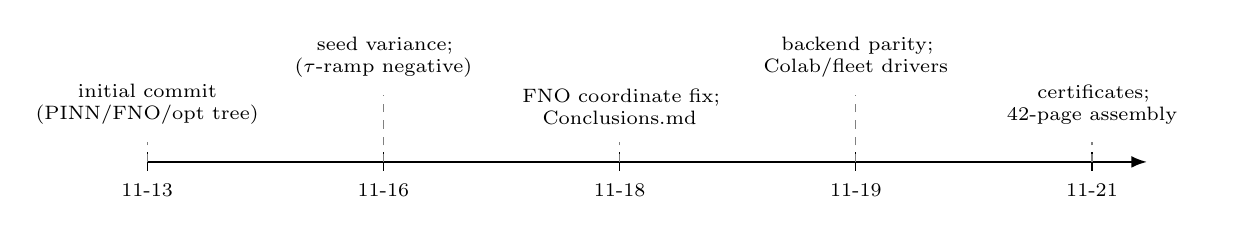
\begin{tikzpicture}[x=1cm,y=1cm,font=\scriptsize]
  \draw[-{Latex[length=2mm]}, thick] (0,0) -- (12.7,0);
  \foreach \x/\d in {0/11-13, 3/11-16, 6/11-18, 9/11-19, 12/11-21} {
    \draw (\x,0.12) -- (\x,-0.12);
    \node[below] at (\x,-0.16) {\d};
  }
  \node[above, align=center, text width=2.8cm] at (0,0.35)
    {initial commit\\(PINN/FNO/opt tree)};
  \node[above, align=center, text width=3.0cm] at (3,0.95)
    {seed variance;\\($\tau$-ramp negative)};
  \node[above, align=center, text width=3.0cm] at (6,0.35)
    {FNO coordinate fix;\\Conclusions.md};
  \node[above, align=center, text width=3.0cm] at (9,0.95)
    {backend parity;\\Colab/fleet drivers};
  \node[above, align=center, text width=3.2cm] at (12,0.35)
    {certificates;\\42-page assembly};
  \draw[gray, dashed] (0,0) -- (0,0.25);
  \draw[gray, dashed] (3,0) -- (3,0.85);
  \draw[gray, dashed] (6,0) -- (6,0.25);
  \draw[gray, dashed] (9,0) -- (9,0.85);
  \draw[gray, dashed] (12,0) -- (12,0.25);
\end{tikzpicture}
\caption{The eight-day span in which the loop ran. The dates are commit dates, not a
claim about effort; the point is the density of findings per day once the gates
and the harness existed.}
\label{fig:timeline}
\end{figure}
Those are not the tasks that make a research career, which is precisely why
they are the ones that get skipped. The rest of the article describes what they
bought.

\subsection{Threats to the method}
\label{sec:method-threats}

The loop is not self-validating. An agent can write a test that encodes the
current bug, a gate with a threshold chosen to pass, or a summary that rounds a
single seed into a trend. The defences used here were procedural, not
architectural: the human set thresholds before seeing results; every merged
mechanism had to fail on a known-bad input; and negative results were recorded
with the same care as positive ones. These defences are fallible, and
\S\ref{sec:discussion} returns to them.

% ======================================================================
% 04-mechanisms.tex — five mechanisms that made the code reusable
% ======================================================================
\section{Five mechanisms that made the code reusable}
\label{sec:mechanisms}

The project has no grand architecture. It has five mechanisms, each of which
was added because a specific failure demanded it. We use the same template for
each: the failure, the mechanism, what it caught, and what it cost.

\subsection{One reference implementation, many backends}
\label{sec:parity}

\paragraph{Failure.} The first GPU backend was a second implementation of the
same physics, and it silently diverged from the NumPy reference on a subset of
scenarios. A policy could pass its own reliability gate on the torch path and
fail it on the reference path---which is exactly what happened later to a
three-well policy (\S\ref{sec:fail3well}).

\paragraph{Mechanism.} NumPy is the reference. The torch modules
(\code{physics/\allowbreak fv2d\_torch.py}, \code{stoch/\allowbreak saa\_torch.py}) are the fast path,
and parity is a test, not a hope. The suite compares not only final fields but
intermediate objects: the upwind operator against a sparse matrix, velocity
against the reference, superposition and fixed-sign linearity, batch-axis
independence, mass balance, and the Krylov report. Tolerances are
$10^{-12}$--$10^{-10}$ for float64 and are tightened or relaxed by dtype, not by
whatever makes the test pass.

\begin{lstlisting}[language=Python,caption={The parity pattern: the same scenario,
two backends, one assertion.},label={lst:parity}]
ref = solve_transport_numpy(scenario, q)
got = solve_transport_torch(scenario, q)
np.testing.assert_allclose(got, ref, rtol=1e-10, atol=1e-12)
\end{lstlisting}

\paragraph{What it caught.} A float32 Krylov breakdown that produced a
non-finite residual for one candidate in a compass sweep; a tail-scenario
divergence where the torch test reliability ($0.9625$) disagreed with NumPy
($0.90$); and a set of CUDA-only bugs that a real L4 run exposed (device
resolution, multi-GPU index, zip path). It also makes the fast path auditable:
the NumPy implementation is the specification, and the torch implementation is
allowed to be different only where the tests say so.

\paragraph{Cost.} Two implementations to maintain. The mitigation is
asymmetry: the reference is optimized for clarity, the fast path for throughput,
and the parity suite is the contract between them.

\subsection{Configuration and manifests}
\label{sec:config}

\paragraph{Failure.} A run whose result was recorded, but whose effective
configuration could not be reconstructed: CLI flags overrode config values, a
missing \code{-{}-config} silently fell back to defaults, and a 3.7\,MB file
literally named \code{True} was produced by \code{-{}-save-model True}.

\paragraph{Mechanism.} Every optimization experiment is a YAML file under
\code{configs/opt/}. A missing config is an error, not a default. Every run
writes a \code{run\_config.json} beside its outputs, recording the effective
configuration, seed, device, dtype, git revision and metrics. The runtime log
(\code{runs/runtimes.jsonl}) adds wall clock and evaluation count.

\begin{lstlisting}[caption={The manifest is the run's identity card.}]
{
  "git": "1868f33",
  "seed": {"train": 17000, "test": 710000},
  "device": "cuda", "dtype": "float32",
  "grid": [160, 96], "nsteps": 100,
  "optim": {"max_iter": 5, "init_fraction": 0.1},
  "metrics": {"test_mean_J": 428579.0, "test_reliability": 0.975}
}
\end{lstlisting}

\paragraph{What it caught.} The difference between ``reproduce this run'' and
``reproduce something like this run''. It also exposed a false negative: two
replicas with different \code{optim.seed} but \code{n\_starts=1} were identical,
because the start index consumed no RNG. That observation changed the
multi-replica protocol.

\paragraph{Cost.} One file per run. The benefit is that a result can be
re-derived from its own directory, without a conversation or a memory of which
flags were used.

\subsection{Gates, not assertions}
\label{sec:gates}

\paragraph{Failure.} ``The forward model works'' is not a testable statement.
Neither is ``the optimizer converged''. Without a threshold and an artifact,
both are opinions.

\paragraph{Mechanism.} Each physical assumption is a named gate with a
threshold and an output. The 2D stack has O0--O4 (analytical flow, retained
variance and reproducibility, mass balance and the uniform-pumping limit,
adjoint gradient check, and the three chance-constraint formulations); the 2D
physics has G2.1--G2.5; the 3D stack has six gates including a fresh-scenario
reliability gate. The gate tables are reproduced in Appendix~\ref{app:gates}.

\begin{table}[htbp]
\centering
\small
\begin{tabularx}{\textwidth}{@{}llX@{}}
\toprule
Gate & Threshold & What it protects \\
\midrule
O0 & Thiem head $6.9\times10^{-3}$; velocity $1.4\times10^{-12}$ &
The flow solve is the analytical solution before any wells are added. \\
O1 & retained variance $\ge0.95$; reproducible &
The KL truncation represents the field it claims to represent. \\
O2 & mass balance $\le1\%$; uniform $q$ beats no-pump &
The transport solve conserves mass and the objective is monotone in the
expected direction. \\
O3 & adjoint relative error $\le10^{-6}$ &
The gradient is the gradient of the implemented objective. \\
O4 & all formulations select the same policy &
The chance-constraint reformulations agree where the problem is non-degenerate. \\
G3 & reliability $\ge1-\alpha-1\%$ on held-out scenarios &
The policy is safe on fields it did not optimize on. \\
\bottomrule
\end{tabularx}
\caption{A sample of the gate suite. The full definitions are in
Appendix~\ref{app:gates}; artifacts are under \code{out/opt/hydrology\_gpu\_gates/}
and \code{out3d\_colab/run\_paper/}.}
\label{tab:gates}
\end{table}

\paragraph{What it caught.} A feasible-region saturation that made O4
uninformative on one config; a transport Krylov residual that passed at
$M=8$ but failed at $M=100$; and a final-test reliability gate that passed on
torch and failed on NumPy. The gate did not prevent the bug; it made the bug
visible before a paper did.

\paragraph{Cost.} Gates are code, and they need their own maintenance. The
project keeps them cheap by making each one a script/flag on an existing driver
rather than a separate framework.

\subsection{Statistics as infrastructure}
\label{sec:stats}

\paragraph{Failure.} At fixed hyperparameters the 1D PINN baseline spans
$1.17\times10^{-2}$ to $8.14\times10^{-2}$ across five seeds. A single run is
not a result; a single-seed comparison can invert the sign of a real effect.

\paragraph{Mechanism.} \code{SCRIPTS/seed\_sweep.py} runs any command across a
seed range, pulls one scalar per run from that run's JSON manifest, and reports
median, IQR, min--max and spread. For two arms it performs a \emph{paired}
comparison on shared seeds and refuses to compare unpaired runs. The decision
rule is encoded: a variant counts only if it beats the baseline median by more
than the baseline IQR. The harness prints the spread next to every median, so a
claimed improvement is always read against the noise it must beat.

\begin{lstlisting}[caption={The harness makes the statistical rule executable.}]
$ ./SCRIPTS/seed_sweep.py --arm base --seeds 0-4 \
    --metric metrics.regions.full --outdir runs/sweeps/base -- \
    python3 -u SCRIPTS/solve_1d_pinn.py --hard-bc --eps 1e-3 \
      --outdir {outdir}/s{seed} --save-model {outdir}/s{seed}/model.pt
...
median 1.613e-02   IQR 2.175e-02   min 1.171e-02   max 8.144e-02   spread 7.0x
\end{lstlisting}

\paragraph{What it caught.} The $\tau$-ramp result: seed 0 showed a 32--45\%
improvement on every region, but across five paired seeds the ramp won only
two, with a median ratio of $1.31$ in the wrong direction ($p=0.38$). The
harness turned a publishable-looking win into a negative result before it was
published. It also produced the honest FNO number: the single-seed $1.46\%$ at
250 epochs became a five-seed median of $3.02\%$ at 120 epochs
(IQR $3.2\times10^{-3}$).

\paragraph{Cost.} Five runs instead of one. On CPU that is minutes; on a GPU it
is a budget decision, which is exactly the decision that should be explicit.

\subsection{Artifact-first remote execution}
\label{sec:remote}

\paragraph{Failure.} A Colab cell streams its output only when it returns. A
two-hour run therefore looks silent, and a run that dies takes its
\code{/content} directory with it. One run completed an entire start and then
died on a Krylov breakdown; \code{-{}-zip-results} ran only after a successful
dispatch, so nothing was uploaded.

\paragraph{Mechanism.} Three changes make the run, not the process, the unit:
\begin{enumerate}
  \item \textbf{Zip in \code{finally}.} \code{zip\_results\_safely} zips
        whatever exists and never masks the real exception.
  \item \textbf{Read the remote log, not the cell.} A shared helper pulls a
        live run's log with \code{colab download}, a filesystem read that does
        not queue behind the running cell, so a live run reports
        \code{iter 9/40, 163/500 evals, 32.6\%} instead of ``quiet''.
  \item \textbf{Re-score out of sample.} \code{check\_tail.py} re-evaluates a
        finished policy on fresh scenarios, with a separate seed base, and
        reports a Wilson interval. The certificate is not the run's own summary.
\end{enumerate}

\begin{lstlisting}[language=Python,caption={The zip belongs in a \code{finally},
and the zip error must not replace the real one.}]
try:
    zip_results(args)
except Exception as exc:          # never mask the real failure
    print(f"warning: could not zip results: {type(exc).__name__}: {exc}")
\end{lstlisting}

\paragraph{What it caught.} The artifact loss above; a live run that was
mistaken for idle; and a certificate that looked strong in-run
($\Cvar_{5\%}(G)=+0.005$) but moved to $+0.616$ on scenarios no run had seen.
The last is the most important result in the article: the run's own tail
statistic is a property of the sample it optimized on.

\paragraph{Cost.} Remote downloads are slower than reading a local file, so
pulls are bounded (30\,s, one retry) and limited to replicas that are actually
running. The local view is the fallback, with the reason shown inline.

% ======================================================================
% 05-failures.tex — each defect becomes a permanent guard
% ======================================================================
\section{Failure catalogue: each defect becomes a guard}
\label{sec:failures}

The mechanisms in \S\ref{sec:mechanisms} are abstractions. This section is the
evidence that they were not designed in advance: each one is the residue of a
specific failure, and each failure left a test, a flag, a gate or a line in the
memory files. The catalogue is the empirical heart of the article because it is
where the AI contribution is visible as \emph{work done}, not as a claim.

\begin{table}[htbp]
\centering
\small
\begin{tabularx}{\textwidth}{@{}p{3.2cm}p{3.4cm}Xp{1.4cm}@{}}
\toprule
Symptom & Root cause & Permanent guard & Commit \\
\midrule
FNO rel.\ $L^2=0.973$, worse than zeros &
Constant input channels $\Rightarrow$ only the DC mode; output constant by
construction &
Coordinate channels + trivial-predictor guard (all-zeros and mean-field
baselines) &
\code{aadc3fe} \\
One non-finite candidate kills a two-hour run &
A single float32 Krylov breakdown treated as fatal &
\code{-{}-allow-nonfinite} maps one candidate to $+\infty$; a whole sweep still
raises; count is reported &
\code{4e506b1} \\
A dying run uploads nothing &
Zip ran only after a successful dispatch &
\code{zip\_results\_safely} in \code{finally}; zip failure never masks the real
error &
\code{4e506b1} \\
Assembled thesis aborts on \code{remark} &
Preamble merger kept \code{\textbackslash newcommand} only; \code{\textbackslash
newtheorem} and \code{\textbackslash newcolumntype} dropped &
Declarations keyed by declared name; four compiler-only defects pinned by tests &
\code{12dcebf}, \code{3628b5d} \\
$\tau$-ramp looks like a 32\% win on seed 0 &
Single-seed comparison against a 7$\times$ spread &
Paired five-seed sweep; median ratio 1.31 the wrong way; negative result kept &
\code{ecf9537} \\
Three-well policy passes torch reliability 0.9625, fails NumPy 0.90 &
Tail scenarios diverge between backends; SAA overfits its own tail &
Re-score on the NumPy reference before reporting; four wells is the robust
frontier &
\code{6cb9827} \\
$\max|\mathcal{R}|=10^{3}$ looks like a physics error &
Hard-BC ramp contributes $s'(0)=1/\varepsilon$ independently of weights &
Report $1/\varepsilon$ as the reference; use band means, not a global maximum &
\code{bb95c08} \\
``$5\times$ GPU speedup'' is unmeasured &
Launch count assumed, not instrumented &
Instrument the kernel: 4{,}022 matvecs/evaluation, 1.7$\times$ the assumption &
\code{75bbb5a} \\
A100 no faster than a T4 &
Cost is fixed launch overhead, not arithmetic throughput &
Report the regime and the measurement, not the accelerator name &
\code{b1346b5} \\
\bottomrule
\end{tabularx}
\caption{Failure catalogue. Each row is a defect that became a permanent guard.
The commit is the one that introduced the guard, not necessarily the one that
introduced the bug.}
\label{tab:failures}
\end{table}

\subsection{The FNO was structurally incapable}
\label{sec:failfno}

The recorded result was a relative $L^2$ error of $0.973$ on a two-sample test
set. Because the metric is normalized by the target norm, a predictor of all
zeros scores exactly $1.0$: the operator was worse than nothing. The diagnosis
was not ``train longer''. The input was two spatially constant channels
$(v,D)$ broadcast over the grid; the lifting layer is pointwise and every
spectral layer multiplies Fourier coefficients, so a constant input has only the
DC mode and the output is constant by construction. The measured output spatial
standard deviation was $\approx2\times10^{-10}$.

The proof was a constant-input test, not an argument. The fix was to append
normalized $(\xi,\tau)$ coordinate channels---standard practice for FNOs
\citep{li2020fourier}---with a \code{-{}-no-coords} ablation. The result moved from
$0.973$ to $0.0146$ (250 epochs, single seed); a five-seed median at 120 epochs
is $3.02\times10^{-2}$ (IQR $3.2\times10^{-3}$), and the profile-only error
dropped from $1.000$ to $0.071$. The permanent guard is a trivial-predictor
check that prints the all-zeros and mean-field baselines and warns when a run
fails to beat them.

The lesson generalizes: a metric without a trivial baseline can hide a model
that has learned nothing. The guard is four lines and it would have caught the
bug on day one.

\subsection{One bad candidate, one dead run}
\label{sec:failkrylov}

A compass sweep evaluates $2n_w$ candidates per iteration. In mixed float32, a
batched transport Krylov solve occasionally returns a non-finite residual for
one candidate. The original code raised, which is correct for a broken solve but
wrong for one unlucky candidate: a run that had already completed a full start
died at candidate 5 of 18 of the next.

The fix is a policy, not a try/except. \code{nonfinite\_policy} replaces the
offending entries with $+\infty$ when \code{-{}-allow-nonfinite} is set. The
compass acceptance test is \code{fc < best - 1e-12}, so $+\infty$ can never be
accepted: the move is skipped and the sweep continues. A whole batch coming back
non-finite still raises, because that is the batched solve diverging, not one
candidate. The count is reported in the metrics, and \code{multi\_start} still
raises if every start ends non-finite, so a broken backend cannot be silently
tolerated.

The same run exposed the artifact problem: \code{-{}-zip-results} ran only after a
successful dispatch, so start 1's \code{out/} died with the VM and
\code{colab download} reported ``File or directory not found''. The zip now runs
in a \code{finally}, and \code{zip\_results\_safely} never masks the real
exception. Fourteen tests pin both behaviours.

\subsection{Static checks cannot see a preamble}
\label{sec:failbuild}

Assembling the thesis from six standalone chapters looked like a file-merge
problem. The offline checker validated braces, environments, references,
duplicate labels and graphics paths. It passed. A real LaTeX toolchain then
found four defects the checker could not see: \code{natbib} and \code{geometry}
were emitted once per chapter so package options clashed; the preamble merger
carried only \code{\textbackslash newcommand}, dropping
\code{\textbackslash newtheorem\{remark\}} and \code{\textbackslash
newcolumntype\{Y\}}, so the first \code{remark} aborted the build; a two-line
\code{\textbackslash title} leaked its continuation into the preamble; and five
chapters each shipped a \code{thebibliography}, so \code{ogata1961solution}
appeared three times and every citation was ``multiply defined''.

Each defect is now pinned by a test in \code{tests/test\_build\_tex.py}, and the
preamble merger reports a conflict when two chapters define the same name
differently rather than silently choosing one. The general lesson is the one the
article keeps returning to: a check that only reads the source is weaker than a
check that runs the compiler.

\subsection{The negative result that justified the harness}
\label{sec:failtau}

Causal $\tau$-ramping was supposed to shrink the corner band without hurting the
interior. On seed 0 it looked like a large win: full-grid error
$1.42\times10^{-2}\to9.57\times10^{-3}$, interior $8.3\times10^{-3}\to
4.6\times10^{-3}$, improvements on every region. A single-seed sweep would have
``confirmed'' the hypothesis.

Across five paired seeds the ramp won two, and the median ramp/baseline ratio
was $1.31$---worse---with a permutation test $p=0.38$. The baseline alone spans
$1.17\times10^{-2}$ to $8.14\times10^{-2}$ at fixed hyperparameters. The effect
was noise. The experiment is reported as a negative result, and the harness that
made the repetition cheap is now the project's default for any comparison.

This is also the clearest example of the collaboration's value. The agent did
not have a better idea about $\tau$-ramping. It ran the same experiment four more
times and tabulated it, which is the thing a human under deadline pressure
skips.

\subsection{The policy that passed its own gate}
\label{sec:fail3well}

The 160$\times$96 optimization settled on a three-well policy at
$5\ \mathrm{m^3/d}$ per well with test cost $J=419{,}550$ and reliability
$0.9625$ on the torch path---above the $0.94$ gate. Re-scored on the NumPy
reference, the same policy gave $J=419{,}279$ and reliability $0.90$, which
fails. The tail scenarios diverged between backends: $M=8$ parity was exact,
but some high-pumping tail scenarios were not.

The robust frontier is four wells at $J=437{,}964$ and reliability $0.975$,
about 4\% more expensive than three wells and still 16\% cheaper than uniform
$5\ \mathrm{m^3/d}$. The permanent rule is that any three-well policy must be
re-scored on NumPy before it is reported. The deeper lesson is about SAA: with
$M_{\text{train}}=40$, the optimizer can overfit the very tail the chance
constraint is supposed to control.

\subsection{The residual maximum is not a physics error}
\label{sec:failres}

The hard-BC ansatz has $u_\tau$ carrying $s'(\tau)=e^{-\tau/\varepsilon}/
\varepsilon$, so at the corner $|R|=1/\varepsilon=10^{3}$. It is identical at
initialization and after training, and on every seed. The first reading was
``the residual is huge at the inlet''; the correct reading is ``the ansatz has a
structural floor, and a global maximum is the wrong diagnostic''. The fix was
documentation and a band-mean diagnostic, not a code change. This is a case
where the artifact was correct and the interpretation was wrong---the opposite
failure mode from the FNO.

\subsection{Measure the claim before optimizing it}
\label{sec:failcost}

The optimization plan assumed roughly $2{,}400$ batched matrix--vector products
per evaluation and a $5\times$ speedup from removing per-step kernel launches.
Instrumenting \code{bicgstab\_solve} found $4{,}022$ matvecs per evaluation,
$40.2$ per solve, $1.7\times$ the assumption. The speedup may still be available,
but it cannot be claimed until the arithmetic change is implemented and the
parity gate passes. A related measurement killed the accelerator assumption: at
this geometry an A100 was \emph{no faster} than a T4, because the cost is fixed
launch overhead rather than arithmetic throughput. The guard is cultural and now
explicit in \code{Conclusions.md}: do not land an unmeasured speedup.

% ======================================================================
% 06-results.tex — results that survive re-derivation
% ======================================================================
\section{Results that survive re-derivation}
\label{sec:results}

The point of the mechanisms is not tidiness. It is that some claims now survive
attempts to break them, and the ones that do not are labelled. This section
reports the survivors and the caveats together; the full tables are in
Appendix~\ref{app:tables}.

\subsection{One dimension: the baseline is honest, the FNO is fixed}
\label{sec:res1d}

Figure~\ref{fig:1d} shows the PINN against the Ogata--Banks reference. The
qualitative agreement is not the result; the result is the table.

\begin{figure}[htbp]
\centering
\includegraphics[width=0.48\textwidth]{figs/field.png}\hfill
\includegraphics[width=0.48\textwidth]{figs/profiles.png}
\caption{1D sandbox: concentration field and outlet profiles for the hard-BC
PINN against the analytical reference. Generated by \code{SCRIPTS/hydrology.py}
and \code{SCRIPTS/solve\_1d\_pinn.py}.}
\label{fig:1d}
\end{figure}

\begin{table}[htbp]
\centering
\small
\begin{tabular}{lccccc}
\toprule
 & median & IQR & min & max & spread \\
\midrule
$E_{\mathrm{rel}}$ (full grid) & $1.61\times10^{-2}$ & $2.18\times10^{-2}$ & $1.17\times10^{-2}$ & $8.14\times10^{-2}$ & $7.0\times$ \\
$E_{\mathrm{rel}}^{\mathrm{int}}$ ($\xi,\tau>0.05$) & $1.42\times10^{-2}$ & $2.59\times10^{-2}$ & $6.64\times10^{-3}$ & $8.16\times10^{-2}$ & $12.3\times$ \\
\bottomrule
\end{tabular}
\caption{Phase 1 hard-BC baseline over five seeds. The distribution is
right-skewed (mean $3.19\times10^{-2}$, twice the median), so median and IQR are
reported. Artifact: \code{runs/sweeps/baseline\_n5}; harness:
\code{SCRIPTS/seed\_sweep.py}.}
\label{tab:1d}
\end{table}

Two corrections follow from Table~\ref{tab:1d}. First, the corner-excluded
metric does not rescue the target: the best seed
($6.64\times10^{-3}$) is below $10^{-2}$, the median ($1.42\times10^{-2}$) is
not. Second, the corner is not the governing artefact: the two metrics are
rank-correlated (Spearman $\rho=1$), and their ratio ranges from $0.57$ to
$1.00$, so excluding the corner never reorders the runs.

The FNO results are reported with the same discipline. The original operator
scored $0.973$ (worse than zeros); with coordinate channels and 250 epochs it
scored $0.0146$ on one seed. At 120 epochs across five seeds the median is
$3.02\times10^{-2}$ (IQR $3.2\times10^{-3}$, range $2.35\times10^{-2}$ to
$5.98\times10^{-2}$). The honest 120-epoch figure is therefore about 3\%, not
1.5\%; the 250-epoch number still needs its own multi-seed median before it is
quoted as a result. Mode truncation is monotone (modes 4/12/24 $\to$
2.79/2.35/2.19\%, single seed), and resolution invariance degrades gracefully
(train 64$^2$ $\to$ 4.14\%, train 32$^2$ $\to$ 6.92\%, evaluated at
128$^2$), which is the behaviour a genuine operator should show.

\subsection{Two dimensions: two policies, one certificate}
\label{sec:res2d}
\label{sec:res3dcert2d}

The $160\times96$ benchmark is a $200\times120$\,m aquifer, log-normal
conductivity ($\sigma=0.65$, $\ell=15$\,m, $n_{KL}=1529$), nine candidate wells,
$M_{\text{train}}=100$ and $M_{\text{test}}=40$. Two runs used the same search
and differ only in floating-point precision.

\begin{table}[htbp]
\centering
\small
\caption{Two independently certified optima of the same benchmark. Both satisfy
every gate; they differ by 1.2\% in cost while using different well subsets.}
\label{tab:2d}
\begin{tabular}{lrr}
\toprule
 & float64 & float32 (mixed) \\
\midrule
$\mathbf{q}^\star$ [$\mathrm{m^3/d}$] & $(0,9.72,5.86,0,3.38,0,0,0,0)$ & $(0,9.33,8.16,0,0,0,0,0,0)$ \\
total pumping & $19.0$ & $17.5$ \\
active wells & $3$ & $2$ \\
$J$ (train / test) & $433{,}945$ / $434{,}008$ & $428{,}592$ / $428{,}579$ \\
$\Cvar_{5\%}(G)$ (train / test) & $+0.018$ / $-0.007$ & $+0.005$ / $+0.009$ \\
reliability (train / test) & $0.990$ / $0.975$ & $0.990$ / $0.975$ \\
holdout during search & $1.000$ & $0.975$ \\
max.\ mass-balance error & $4.2\times10^{-11}$ & $2.3\times10^{-5}$ \\
wall clock (T4) & $4.14$\,h & $1.67$\,h \\
\bottomrule
\end{tabular}
\end{table}

Two facts matter more than the numbers. Both optima sit \emph{on} the
constraint ($\Cvar\approx0$ from either side), which is what the solution of a
chance-constrained program must do: they are the cheapest policies that are
still safe, not policies that happen to be safe. And the two policies differ by
1.2\% in cost while using different well subsets, so near the optimum the
objective is flat along ``which wells carry the duty''. Replicas with offset
scenario seeds reproduce the same policy digit for digit, which is why the flat
direction is a property of the cost model, not of sampling noise.

\begin{table}[htbp]
\centering
\small
\caption{Out-of-sample certificate on 400 scenarios with 95\% Wilson intervals.
Both clear the $1-\alpha-1\%=0.94$ gate, but not equally. A fresh draw from a
seed no run saw leaves the cost intact and moves the tail.}
\label{tab:cert}
\begin{tabular}{lrrr}
\toprule
policy & violations & reliability & 95\% Wilson CI \\
\midrule
float64 $\mathbf{q}^\star$ & $1/400$ & $0.998$ & $[0.986,\ 1.000]$ \\
float32 $\mathbf{q}^\star$ & $7/400$ & $0.983$ & $[0.964,\ 0.991]$ \\
\bottomrule
\end{tabular}
\end{table}

Table~\ref{tab:cert} is the strongest evidence in the article because it is the
one that does not come from the run's own summary. On scenarios drawn from seed
900000, which no run had seen, the float32 policy gives $J=428{,}509$ against
the run's $428{,}592$ (0.02\% apart), reliability $391/400=0.978$ with Wilson
$[0.958,0.988]$, and $\Cvar_{5\%}(G)=+0.616$ instead of $+0.005$. The policy is
safe; the tail it reported is a property of the sample it optimized on. The same
draw at $M=100$ gives $4/100=0.960$ with a Wilson interval of $[0.902,0.984]$,
which is inconclusive: the search's own sample size cannot certify the policy it
produced. Figure~\ref{fig:certificate} makes that argument visual: the intervals
only resolve the two policies at $M=400$.

\begin{figure}[htbp]
\centering
\includegraphics[width=0.58\textwidth]{figs/reliability_certificate.png}
\caption{Empirical reliability with its 95\% Wilson interval as a function of the
number of out-of-sample scenarios, for both certified policies (drawn on the
host run's test seeds; the seed-900000 draw above is the independent check). At
$M\le100$ the intervals overlap, straddle the $0.94$ gate and cannot separate the
two policies; only at $M=400$ does the weaker one ($0.983$) fall clearly below the
stronger ($0.998$). A point estimate of $0.975$ at $M=40$ is consistent with a
true reliability anywhere in $[0.87,1.00]$, which is why the certificate is
quoted as an interval. Generated by \code{SCRIPTS/make\_figures.py} from the
\code{check\_tail.py --ladder} output.}
\label{fig:certificate}
\end{figure}

\paragraph{A cheaper policy that fails the audit.} The certificate above is
built from policies a search \emph{accepted}. The complementary case is a
deliberately weaker search: the same objective at $160\times96$ with
$M_{\text{train}}=M_{\text{test}}=M_{\text{holdout}}=40$, two starts, 400
evaluations per start, float32 with the float64 Krylov recurrence, run twice on
different random seeds (7 and 8) so that only the starting points differ.
Table~\ref{tab:restart} is the result.

\begin{table}[htbp]
\centering
\small
\caption{Restarts do not find a second optimum at $M_{\text{train}}=40$; they
find the same fragile one twice. Both replicas optimise the same 40-scenario
objective, so the only difference between them is the starting points.}
\label{tab:restart}
\begin{tabular}{lrrrrl}
\toprule
replica & start 1 (det.) & start 2 (random) & $\mathbf{q}^\star$ & train / test rel. & verdict \\
\midrule
seed 7 & $409{,}863$ & $421{,}639$ & $[2.59,0,9.72,0\ldots]$ & $0.975$ / $0.900$ & fails \\
seed 8 & $409{,}863$ & $415{,}576$ & $[2.59,0,9.72,0\ldots]$ & $0.975$ / $0.900$ & fails \\
\bottomrule
\end{tabular}
\end{table}

Both random starts converged \emph{worse} than the deterministic one, so both
replicas returned the identical $\mathbf{q}^\star$ ($12.32\ \mathrm{m^3/d}$ from
two wells): at this sample size the landscape has one dominant attractor, and it
is the fragile policy. On the seed-900000 draw the same audit that passed the two
certified policies reports $J=409{,}645$---$4.4\%$ cheaper than the accepted
policy---with $34/400$ violations, reliability $0.915$ and Wilson
$[0.884,0.939]$, an interval entirely below the gate. The violation count grows
with the sample ($0/16$, $1/20$, $2/40$, $3/60$, $5/100$, $6/150$, $13/200$,
$28/300$, $34/400$), the opposite of the accepted policies, whose count stays
flat while the tail mean drifts; under-sampling can hide violations or exaggerate
them, so the sign is not predictable and the sample cannot be sized by watching
$\Cvar$.

The failure is statistical, not numerical. The 802 evaluations produced no
non-finite objective and no stalled solve, so float32 at $M=40$ did its job and
the sample size did not. This is also the first live catch for the mid-run
guard: a disjoint holdout archive, re-evaluated every eight sweeps at about $1\%$
of a sweep's cost, reported $\text{rel}=0.900$ and $\Cvar=+1.63$ at iteration 16
on \emph{both} replicas, and again at iteration 24---turning a post-mortem into an
abort decision while the VM was still running.

Figure~\ref{fig:plume} shows what the policy does to the plume. On 80 held-out
scenarios the float64 policy lowers the peak concentration from $35.81$ to
$0.433\ \mathrm{mg/L}$ (median, IQR $-97.4\%$ to $-99.3\%$) and the
compliance-point concentration from $17.23$ to $0.0260\ \mathrm{mg/L}$, raising
the number of scenarios meeting the $1.0\ \mathrm{mg/L}$ limit from $1/80$ to
$78/80$. The plume is displaced rather than erased: its peak moves
down-gradient to $x\approx115$\,m, adjacent to the active well.
Figure~\ref{fig:chance} shows the tail of the violation distribution that these
medians average over.

\begin{figure}[htbp]
\centering
\includegraphics[width=0.88\textwidth]{figs/contamination.png}
\caption{Untreated contamination and the certified policy on the 2D benchmark.
Each panel carries its own colour scale so the cleaned field is visible; active
wells are annotated with their rates. Artifact:
\code{out/certified\_20261120-111849/figures/contamination.png}.}
\label{fig:plume}
\end{figure}

\begin{figure}[htbp]
\centering
\includegraphics[width=0.92\textwidth]{figs/chance_tail.png}
\caption{The constraint behind the certificate, at $M=40$ out-of-sample
scenarios and the float64 policy. (a) The distribution of the worst
compliance-point violation $G$: 39 scenarios sit at the $\sim-1$ floor because the
plume is fully captured, one violates. The priced $\Cvar_{5\%}(G)\approx0$ -- the
policy sits exactly on the constraint, as the solution of a chance-constrained
program must. (b) Cleanup time: $0$\,d for 39/40 scenarios, the horizon cap for the
single violating one. Generated by \code{SCRIPTS/make\_figures.py}.}
\label{fig:chance}
\end{figure}

\subsection{Three dimensions: verified first, and that is how the bug was found}
\label{sec:res3d}

The 3D runner is a self-contained NumPy/SciPy implementation (TPFA Darcy,
diagonal Bear dispersion, vertical anisotropy, partially penetrating wells) with
pattern search and multiple starts. Before quoting any of its numbers we asked
it questions whose answers do not depend on our own code, and that turned out to
matter more than expected.

Two checks are now permanent tests. The first is a \emph{moment} test: put a
pulse in the middle of the domain and read the growth of its spatial variance.
It must obey $\mathrm{Var} = 2Dt$ with the coefficients the operator claims to
assemble, and it does --- longitudinal $D = \alpha_L v + v\Delta x/2$ (the
second term is the first-order upwind contribution, recovered to $10\%$),
transverse $D = \alpha_T v$ on both axes, and a centroid drifting at the pore
velocity $v = K\,\mathrm{grad}/\phi$ rather than the Darcy velocity. The second
is a \emph{front} test against Ogata--Banks. A mass-flux inlet is not a Dirichlet
inlet: the classical formula carries a reflected term
$\mathrm{e}^{vx/D}\operatorname{erfc} b$ that a purely advective inlet has no
analogue for, and at the parameters used here the two solutions differ by a
\emph{shift} of $D/v$ --- five to ten cells, independent of $\Delta x$. Against
the correct reference, the swept front
$\tfrac12 C_0\operatorname{erfc}\big((x-vt)/2\sqrt{Dt}\big)$, the interior
relative $L^2$ error is $1.1\times10^{-2}$ at $\Delta x = 1$\,m and
$4.0\times10^{-3}$ at $\Delta x = 0.5$\,m: first order in $\Delta x$, inside the
$1.5\times10^{-2}$ gate. The $0.41$ ``shape error'' we had been carrying was the
wrong reference, and no amplitude fit could have revealed that, because the
mismatch is a shift rather than a scale.

Writing those tests is what exposed a real defect. The 3D fields are stored
$(n_z, n_y, n_x)$, but \code{Grid3D.centres()} returned
\code{meshgrid(x, y, z)} --- that is, $(n_x, n_y, n_z)$ --- and the Gaussian well
kernel is built from those arrays and then flattened. Every well was therefore
written into a transposed cell: on a cubic check grid a well requested at
$(3.5, 2.5, 2.0)$ landed at $(0.5, 2.5, 3.5)$. No run could reveal it, because
the coordinates reported in \code{metrics.json} are the \emph{requested} ones and
the z-screen mask was applied to a coordinate array that was itself transposed.
Every 3D result before 2026-11-23 describes a well layout nobody specified. The
fix is three lines and two regression tests that ask where the kernel actually
peaks; the corrected results are in Section~\ref{sec:res3dcert}. We report the
episode because it is the argument for the protocol rather than against it: the
audit could not have found this, and neither could a parity test between the
NumPy and torch paths, which agreed with each other because both were wrong in
the same way. Only an outside reference could.

\begin{table}[htbp]
\centering
\small
\caption{3D presets after the well-placement fix. The paper preset now settles
on two wells, not four, and is $18\%$ cheaper.}
\label{tab:3d}
\begin{tabular}{lrrrr}
\toprule
preset & grid & $n_{KL}$ & scen.\ (tr/te) & result \\
\midrule
smoke & $12\cdot6\cdot3=216$ & 164 & 6/12 & degenerate: already compliant, $q^\star=0$ \\
paper & $32\cdot16\cdot8=4096$ & 1419 & 64/128 & $q^\star=[0,10.64,0,0,0,12.79,0,0,0]$, rel.\ $0.953$ \\
paper & $32\cdot16\cdot8=4096$ & 1419 & 64/128 & train $J=449{,}972$; certified $0.9725$ on 400 fresh fields \\
\bottomrule
\end{tabular}
\end{table}

\begin{figure}[htbp]
\centering
\includegraphics[width=0.46\textwidth]{figs/3d_well_layout.png}\hfill
\includegraphics[width=0.50\textwidth]{figs/3d_convergence.png}
\caption{3D paper preset after the fix: well layout and search convergence.
Artifacts: \code{out3d\_colab/paper\_fixed/figures/}.}
\label{fig:3d}
\end{figure}

\subsection{Two certified 3D policies, and what multiplicity looks like}
\label{sec:res3dcert}

The paper preset resolves the $20$\,m correlation length with $2.4$ cells, so a
second 3D geometry was run at $40\times20\times10=8{,}000$ cells
($\Delta x=\Delta y=5$\,m, $\Delta z=2$\,m, $n_{KL}=2062$), where the same
correlation length spans four cells and the screened interval covers three
layers, so partially penetrating wells produce real vertical flow. Every policy
below was audited on 400 fresh fields (seed base $900{,}000$) that no search had
seen.

\begin{table}[htbp]
\centering
\footnotesize
\caption{Corrected 3D results. Every row is a different search, and each was
audited on 400 fresh fields. The two $0.97$ rows are certified; the $M_{\text{train}}
=24$ row is the cheapest and inconclusive, and the NumPy row has the best in-run
number of any 3D run and still does not certify.}
\label{tab:3dcert}
\begin{tabular}{llrrrr}
\toprule
geometry & search & $q^\star$ (m$^3$/d) & train $J$ & in-run & 400-field rel.\;[CI] \\
\midrule
$8{,}000$ & torch T4, $M{=}24$  & $[0,0,12.5,0,0,8.59]$ & $441{,}298$ & $0.958$ & $0.9375$;\;[0.909, 0.957] \\
$8{,}000$ & torch T4, $M{=}40$  & $[0.05,12.5,0,0,10.06,0]$ & $446{,}742$ & $0.979$ & $0.9700$;\;[0.948, 0.983] \\
$8{,}000$ & torch T4, $M{=}100$ & $[0.2,12.5,0,0,9.77,0]$ & $446{,}286$ & $0.979$ & $0.9700$;\;[0.948, 0.983] \\
$4{,}096$ & torch T4, $M{=}64$  & $[0,10.64,0,0,0,12.79,0,0,0]$ & $449{,}972$ & $0.953$ & $0.9725$;\;[0.951, 0.985] \\
$4{,}096$ & NumPy, 3 starts    & $[17.05,0,0,0,0,0,0,0,8.42]$ & $457{,}397$ & $0.984$ & $0.9475$;\;[0.921, 0.965] \\
$13{,}824$ & torch T4, $M{=}40$ & $[12.7,0,0,0,0,9.28]$ & $445{,}090$ & $0.938$ & $0.9500$;\;[0.924, 0.967] \\
\bottomrule
\end{tabular}
\end{table}

Three things follow, and the first corrects an earlier draft of this section.
\emph{The $M_{\text{train}}=40$ failure was an artefact of the transposed wells.}
Before the fix, that search found a cheaper policy which audited at $0.9050$ and
looked like the two-dimensional story repeating. At the corrected geometry the
same search finds the $M_{\text{train}}=100$ policy to $0.1\%$ and both certify
at $0.970$; the reading of the earlier failure is withdrawn. A weaker boundary
does remain: $M_{\text{train}}=24$ ($\alpha M_{\text{train}}=1.2$) is the cheapest
policy in the table, $21.09$\,m$^3$/d at $J=441{,}298$, and it audits at
$0.9375$ with a point estimate under the gate, while $\alpha M_{\text{train}}=2.0$
passes. So cost and reliability are anti-correlated across these policies ---
$1.1\%$ cheaper, $0.037$ lower on the audit --- but the crossover sits between
one and two expected tail samples, lower than the two-dimensional rule of five.
We report the boundary we measured rather than the one we expected.

Second, \emph{policy multiplicity is real and is not a search artifact}. At the
paper geometry two searches with the same seeds and different hardware settled on
different designs: wells $\{2,6\}$ at $10.64$ and $12.79$\,m$^3$/d ($J=449{,}972$,
audited $0.9725$), and wells $\{1,9\}$ at $17.05$ and $8.42$\,m$^3$/d
($J=457{,}397$). Both are plausible engineering answers, $1.6\%$ apart in cost. A
single search is therefore not evidence of a unique optimum, and we do not claim
one.

Third, \emph{the in-run test row is not a certificate}, and the paper geometry
makes that unambiguous. The second design above has the \emph{best} in-run
reliability of any 3D run here --- $0.984$, comfortably above the gate --- and its
$400$-field audit lands at $0.9475$, inconclusive, with a point estimate under the
gate. Had we stopped at the run's own row we would have certified the wrong
policy; the audit reversed the ranking relative to the in-run numbers
($0.984$ versus $0.953$ in-run, $0.9475$ versus $0.9725$ audited).

A larger geometry does not extend either conclusion. At $13{,}824$ cells ($\Delta x=\Delta y=4.17$\,m, $n_{KL}=2706$,
$M_{\text{train}}=40$, $5.8$\,s per evaluation on the same T4, $103$ evaluations in
$613$\,s), extends neither conclusion. It found
$q^\star=[12.7,0,0,0,0,9.28]$\,m$^3$/d at $J=445{,}090$, and the audit returns
$J=445{,}101$ --- the objective reproduces across draws to $0.02\%$ --- with
$20/400$ violations, reliability $0.9500$ and Wilson $[0.924,0.967]$:
inconclusive, point estimate above the gate and lower bound below it. Its in-run
row had already failed ($0.9375$), so on this geometry the smoke detector was
right, which is the reverse of the paper geometry and is exactly why it is only a
smoke detector. What the run does \emph{not} do is transfer the $8{,}000$-cell
certificate ($0.9700$): the grid and the KL realisation change together
($n_{KL}$ 2062 versus 2706), so this is not a resolution study and we do not read
it as one. Cost per scenario keeps growing with cell count --- $0.032$\,s at
$4{,}096$, $0.071$ at $8{,}000$, $0.145$ at $13{,}824$ --- and the run still fits
a twelve-minute VM window.

What made the $100$-scenario search affordable is exactly the lever of
Section~\ref{sec:rescost}: the batched backend evaluates $100$ scenarios in
$7.2$\,s where the NumPy reference needs about $105$\,s, a $15\times$ gain from
replacing $100$ sparse factorisations with one batched Krylov solve. It is not a
property of the card --- CPU torch is already $2.4\times$ faster than NumPy at
this geometry --- and the T4 run cost $697$\,s in total.

\subsection{Cost: the accelerator is not the lever}
\label{sec:rescost}

\begin{table}[htbp]
\centering
\small
\caption{Measured cost levers. The first two are real and reproducible; the
third is a caution.}
\label{tab:cost}
\begin{tabularx}{\textwidth}{@{}lXr@{}}
\toprule
Lever & Measurement & Speedup \\
\midrule
Batch a compass sweep & one kernel call per sweep at $80\times40$, T4, $M=8$ & $47\times$ \\
Mixed float32 & float32 operator, float64 Krylov recurrence, $160\times96$ & $2.46\times$ \\
A100 vs T4 & same geometry; fixed launch overhead dominates & no gain \\
\bottomrule
\end{tabularx}
\end{table}

Table~\ref{tab:cost} is the cost section in one line: batching and precision
are levers, the accelerator name is not. Section~\ref{sec:res3dcert} is what
that advice buys when it is followed: batching a 3D sweep and its scenarios is
what made a $100$-scenario search affordable, and the affordable search is the
one that produced a policy that passes its audit. The workload is latency-bound in
float32 and fp64-throughput-bound in float64, so the choice of accelerator is
regime-dependent rather than monotone in price. The honest conclusion is the
one in \code{DOCS/GPU.md}: do not rent a GPU for this problem until the kernel
launch count is reduced; the measured count is $4{,}022$ matvecs per evaluation,
$1.7\times$ the number the optimization plan assumed. Figure~\ref{fig:compute}
shows the same table as bars, grouped by geometry so that no bar is compared
against a different grid.

\begin{figure}[htbp]
\centering
\includegraphics[width=0.92\textwidth]{figs/compute_cost.png}
\caption{Measured cost, grouped so that every comparison is like-for-like.
(a) One 18-candidate compass sweep. At $80\times40$ float32 the T4 is $47\times$
faster than one NumPy core; at $160\times96$ float64 it is \emph{not faster at
all} ($680$\,s against $662$\,s), and only the A100 wins ($106$\,s, $6.4\times$).
Float32 is launch-overhead-bound and float64 is fp64-throughput-bound, so
``buy an accelerator'' is not one decision. (b) On the T4 the $17\times$ comes
from batching candidates into one kernel call, not from the card. Numbers
measured on rented hardware; see \code{DOCS/GPU.md}.}
\label{fig:compute}
\end{figure}

% ======================================================================
% 07-discussion.tex
% ======================================================================
\section{Discussion: what AI did and did not do}
\label{sec:discussion}

\subsection{Separate the harness from the model}
\label{sec:harness-model}

Public discussions of AI-assisted programming usually compare models on a single
completion: given a prompt, which one writes the better function? That is not the
unit that mattered here. The unit was a \emph{turn}: read the repository, form a
hypothesis, edit, run the gate, record the result. Pi supplied the loop; DeepSeek
supplied the hypothesis. Most of the leverage came from the loop.

Three consequences follow. First, a model that is slightly worse at code
generation but equally good at following a procedure would have produced almost
the same project, because the procedure, not the completion, was the bottleneck.
Second, the value compounds with the repository: the more memory the agent can
read, the fewer turns are wasted re-learning. Third, the failure modes are
process failure modes, not syntax failure modes---a plausible hypothesis that
the gate rejects is the normal case, not an exception.

\subsection{Where the agent was useful}
\label{sec:agent-good}

\begin{itemize}
  \item \textbf{Repetition.} The five-seed $\tau$-ramp sweep exists because running
        it four more times was cheap. The 400-scenario certificate exists
        because re-scoring on a fresh seed was a command, not a project.
  \item \textbf{Parity and regression tests.} Comparing two implementations
        field by field, at several tolerances, on many scenarios, is tedious
        and exactly the kind of work an agent does without drift.
  \item \textbf{Documentation from artifacts.} The run log, the runtime table
        and the conclusions were rebuilt from stored JSON rather than memory,
        which is why the numbers in this article can be traced.
  \item \textbf{Searching the history.} Reconstructing when a claim changed
        across 69 commits is a task a human postpones and an agent performs.
  \item \textbf{Writing the guard.} After each failure, the agent wrote the
        smallest test that would have caught it. The guard is often four lines;
        the discipline is remembering to write it.
\end{itemize}

\subsection{Where the agent was wrong}
\label{sec:agent-bad}

The failure catalogue is also a catalogue of agent errors, and it is worth
naming them:
\begin{itemize}
  \item \textbf{Confident single-seed claims.} The $\tau$-ramp result was reported as
        an improvement before the paired sweep. The prose was plausible; the
        evidence was one seed.
  \item \textbf{Plausible structural fixes.} The FNO fix required proving that
        the old architecture \emph{could not} represent a front. A patch that
        merely trained longer would have been plausible and wrong.
  \item \textbf{Over-broad cleanups.} A ``simplification'' that removes the
        residual chunking is a regression on the 961\,MB host, even though it is
        correct on a GPU box. The memory file had to say so explicitly.
  \item \textbf{Metric drift.} Editing an evaluation script can silently change
        what a number means. The manifests and the artifact paths are the
        defence; a diff review alone is not.
  \item \textbf{Optimism about hardware.} The $5\times$ speedup and the A100
        assumption were both plan-level claims that survived until they were
        instrumented.
\end{itemize}

None of these is exotic. They are the ordinary failure modes of a competent,
tired collaborator. The response is therefore procedural rather than
technological: make the gate cheap, make the number traceable, and make the
negative result as easy to record as the positive one.

\subsection{The human protocol}
\label{sec:protocol}

The project converged on five rules, and they are the part most likely to
transfer:
\begin{enumerate}
  \item \textbf{Set the threshold before seeing the result.} A gate chosen after
        the run is a description, not a test.
  \item \textbf{Demand a failing test first.} A bug fix without a test that
        fails on the old code is a hypothesis, not a repair.
  \item \textbf{Ask what would falsify the claim.} If the answer is ``another
        seed'', run it; if the answer is ``nothing'', the claim is not
        empirical.
  \item \textbf{Keep the negative result.} The $\tau$-ramp, the A100 and the 3-well
        policy are as valuable as the successes, because they stop the project
        from repeating them.
  \item \textbf{Own the final judgement.} The agent can draft the conclusion;
        the human decides whether the evidence class supports it.
\end{enumerate}

\subsection{Threats to validity}
\label{sec:threats}

This is an experience report, not a controlled experiment. The sample is one
project, one human and one agent configuration; the models changed during the
work; there is no baseline project developed without AI; and the author is not
neutral about the outcome. The quantitative results are reproducible from the
repository, but the \emph{causal} claim---that the AI loop caused the
reusability---is an interpretation, supported by the commit history and the
failure catalogue, not by randomization.

Two further caveats are specific to the science. The 3D result is validated at
three presets but not against an independent 3D solver; the 2D certificate is
strong on reliability but shows that the reported CVaR tail does not survive a
fresh draw; and the 1D/FNO medians are five seeds, which is enough to see a 7$\times$
spread but not enough to estimate a tail. These are the same caveats the
repository records in \code{Conclusions.md}, and they are repeated here because
an article that hides them would reproduce the failure it is describing.

\subsection{What would make this a stronger study}
\label{sec:future}

A controlled comparison would need two teams, the same task and the same
deadline, one with and one without an agent, and a pre-registered measure of
reusability (e.g.\ time to reproduce a result on a fresh machine, number of
claims that survive an out-of-sample check). That study is worth doing. In its
absence, the best this article can do is make its own evidence trail complete
enough that a reader can disagree with the interpretation while trusting the
numbers.

% ======================================================================
% 08-conclusion.tex
% ======================================================================
\section{Conclusion}
\label{sec:conclusion}

The project did not become reusable because it acquired a package layout or a
test count. It became reusable because every failure left a guard, every guard
left an artifact, and every artifact was written where the next session would
look. The five mechanisms are the visible residue of that process: one reference
implementation with a parity-tested fast path, manifests that make a run
self-describing, gates that turn physical assumptions into go/no-go decisions, a
statistical harness that makes a single seed embarrassing, and an artifact-first
runner that treats the run rather than the process as the unit.

The scientific results that survive are modest and specific: a 1D baseline
reported as a median with a 7$\times$ spread; an FNO repaired from worse than
zeros to a 3\% median; two 2D policies 1.2\% apart on different well sets with a
400-scenario certificate; and a 3D paper preset reproduced on a third machine.
The results that do not survive are just as useful: $\tau$-ramping, a three-well
policy, a reported CVaR tail, and a planned GPU speedup. Keeping both lists is
the practice.

The AI contribution was real but narrower than the marketing: it made
verification, repetition and record-keeping cheap enough to be habitual. The
human contribution was to decide what counted as evidence. The repository
contribution was to remember. A project that keeps all three---and writes down
which is which---can be reused by someone who was not there.

\paragraph{Code and data availability.}
The repository contains the solvers, configs, tests, run manifests and artifacts
referenced in this article. The reproducibility entry points are
\code{python tests/run\_tests.py}, \code{python SCRIPTS/build\_tex.py
--check-only}, and the per-section commands in Appendix~\ref{app:repro}. The
article source, evidence ledger and source map are in \code{ARTICLE/}.


\bibliographystyle{plainnat}
\bibliography{refs}

\appendix
% ======================================================================
% appendix.tex — gates, repository map, artifacts, reproduction
% ======================================================================
\section{Gate definitions}
\label{app:gates}

A gate is a named threshold on a named artifact. The tables below reproduce the
definitions used in the article; the full text is in
\code{DOCS/2D\_plan.md}, \code{TEX/plans\_2d\_3d.tex} and
\code{DOCS/3D\_results.md}.

\begin{table}[htbp]
\centering
\small
\begin{tabularx}{\textwidth}{@{}lXl@{}}
\toprule
Gate & Condition & Artifact \\
\midrule
O0 & Thiem head relative error $6.89\times10^{-3}$; velocity $1.4\times10^{-12}$ & \code{out/opt/hydrology\_gpu\_gates/} \\
O1 & retained KL variance $0.9500$; $n_{KL}=1529$; reproducible & same \\
O2 & mass balance $7.1\times10^{-15}$; uniform $q=5$ gives $J=529{,}250$, reliability $1.0$; no pump $J=317{,}653$, reliability $0.025$ & same \\
O3 & adjoint relative error $2.6\times10^{-11}$ & same \\
O4 & all three chance-constraint formulations select $q=5$ (saturated region, uninformative on this config) & same \\
G2.1 & extruded 1D interior rel-$L^2\le1.5\times10^{-2}$; wall-normal gradient $\le10^{-3}$ & \code{DOCS/2D\_plan.md} \\
G2.2 & plume-core rel-$L^2\le5\%$; mass balance $\le1\%$ & same \\
G2.3 & head rel-$L^2\le10^{-3}$; velocity rel-$L^2\le10^{-2}$ away from wells & same \\
G2.4 & FV observed order $\ge1.8$; PINN MMS $\le2\times10^{-2}$; held-out $K$ $\le5\%$ & same \\
G2.5 & cleanup-time error $\le10\%$; FNO rollout error $\le5\%$; surrogate $\ge100\times$ & same \\
G3 & KL retained variance $\ge0.95$; reproducible; mass balance $\le1\%$; test reliability $\ge1-\alpha-1\%$; improvement over no pump; no-pump reliability recorded & \code{DOCS/3D\_results.md} \\
\bottomrule
\end{tabularx}
\caption{Gate definitions used by the article. A gate is go/no-go: it has a
threshold, an artifact and a failure mode.}
\label{tab:gates-full}
\end{table}

\section{Repository map}
\label{app:repo}

\begin{table}[htbp]
\centering
\small
\begin{tabularx}{\textwidth}{@{}lX@{}}
\toprule
Path & Contents \\
\midrule
\code{physics/} & Finite-volume flow/transport: NumPy reference and batched torch \\
\code{stoch/} & Random fields, wells, objective, SAA, chance constraints, adjoint, optimizer, report \\
\code{SCRIPTS/} & Entry points: solvers, drivers, sweep harness, remote runner, viewer, build script \\
\code{configs/opt/} & Benchmark, exploration and certificate configurations \\
\code{tests/} & Unit, gradient-check, parity and regression tests \\
\code{DOCS/} & Plans, run log, conclusions, GPU audit, usage guide, article plan \\
\code{TEX/} & Standalone chapters and the assembled thesis build \\
\code{ARTICLE/} & This article: master, sections, figures, evidence ledger, source map \\
\code{out/}, \code{runs/} & Run artifacts, manifests, sweeps, certificates, figures \\
\bottomrule
\end{tabularx}
\caption{Repository layout. The rule is that everything runnable lives in
\code{SCRIPTS/}, the packages hold libraries, and the write-ups live in
\code{DOCS/}.}
\label{tab:repo}
\end{table}

\section{Artifact and seed ledger}
\label{app:tables}

Every quantitative claim in \S\ref{sec:results} is listed here with its seed
count and artifact path. This is the appendix equivalent of the repository's
\code{EVIDENCE.md}.

\begin{table}[htbp]
\centering
\small
\begin{tabularx}{\textwidth}{@{}lXl@{}}
\toprule
Claim & Artifact & Seeds / $N$ \\
\midrule
1D full-grid median $1.61\times10^{-2}$ & \code{runs/sweeps/baseline\_n5} & 5 \\
1D interior median $1.42\times10^{-2}$ & same & 5 \\
FNO 120-epoch median $3.02\times10^{-2}$ & \code{runs/sweeps/fno\_coords\_120ep} & 5 \\
FNO 250-epoch $1.46\%$ & \code{out/fno10} and run artifacts & 1 \\
2D float64 policy $J=434{,}008$ & \code{runs/colab\_multi/20261118-114831} & 40 test \\
2D float32 policy $J=428{,}579$ & \code{out/certified\_20261120-111849} & 40 test \\
2D certificate $391/400$ & \code{out/cert/f32\_M400.json} & 400 \\
2D fresh CVaR $+0.616$ & same, \code{-{}-seed-base 900000} & 400 \\
3D paper preset $J=547{,}665.31$ & \code{out3d\_colab/run\_paper/} & 128 test \\
3D third-machine reproduction & local run, 1014.8\,s & 128 test \\
\bottomrule
\end{tabularx}
\caption{Evidence ledger. A number without a row here does not belong in
\S\ref{sec:results}.}
\label{tab:ledger}
\end{table}

\section{Reproduction commands}
\label{app:repro}

\begin{lstlisting}[language=bash,caption={The commands a reader needs to check
the article's claims.}]
# tests (172 functions across 22 modules)
python tests/run_tests.py

# LaTeX assembly checks (no compiler needed)
python SCRIPTS/build_tex.py --check-only

# 1D baseline, five seeds
./SCRIPTS/seed_sweep.py --arm base --seeds 0-4 \
  --metric metrics.regions.full --outdir runs/sweeps/base -- \
  python3 -u SCRIPTS/solve_1d_pinn.py --hard-bc --eps 1e-3 \
    --outdir {outdir}/s{seed} --save-model {outdir}/s{seed}/model.pt

# 2D gate suite
python SCRIPTS/run_optimization.py --config configs/opt/hydrology_gpu.yaml --stage gates

# 3D paper preset (laptop CPU)
python full3D_colab_run.py --preset paper --budget 15 --n-starts 2

# Re-score a policy on fresh scenarios
python SCRIPTS/check_tail.py --run out/certified_20261120-111849 \
  --m-scen 400 --seed-base 900000
\end{lstlisting}

The article source is built with \code{make} in \code{ARTICLE/}. The evidence
ledger is \code{ARTICLE/EVIDENCE.md}; the source map for material lifted from
\code{TEX/} is \code{ARTICLE/SOURCE\_MAP.md}.


\end{document}
